% Copyright (C) 2014-2020 by Thomas Auzinger <thomas@auzinger.name>

\documentclass[draft,final]{vutinfth} % Remove option 'final' to obtain debug information.

% Load packages to allow in- and output of non-ASCII characters.
\usepackage{lmodern}        % Use an extension of the original Computer Modern font to minimize the use of bitmapped letters.
\usepackage[T1]{fontenc}    % Determines font encoding of the output. Font packages have to be included before this line.
\usepackage[utf8]{inputenc} % Determines encoding of the input. All input files have to use UTF8 encoding.

% Extended LaTeX functionality is enables by including packages with \usepackage{...}.
\usepackage{amsmath}    % Extended typesetting of mathematical expression.
\usepackage{amssymb}    % Provides a multitude of mathematical symbols.
\usepackage{mathtools}  % Further extensions of mathematical typesetting.
\usepackage{microtype}  % Small-scale typographic enhancements.
\usepackage[inline]{enumitem} % User control over the layout of lists (itemize, enumerate, description).
\usepackage{multirow}   % Allows table elements to span several rows.
\usepackage{booktabs}   % Improves the typesettings of tables.
\usepackage{subcaption} % Allows the use of subfigures and enables their referencing.
\usepackage[ruled,linesnumbered,algochapter]{algorithm2e} % Enables the writing of pseudo code.
\usepackage[usenames,dvipsnames,table]{xcolor} % Allows the definition and use of colors. This package has to be included before tikz.
\usepackage{nag}       % Issues warnings when best practices in writing LaTeX documents are violated.
\usepackage{todonotes} % Provides tooltip-like todo notes.
\usepackage{hyperref}  % Enables cross linking in the electronic document version. This package has to be included second to last.
\usepackage[acronym,toc]{glossaries} % Enables the generation of glossaries and lists fo acronyms. This package has to be included last.

% Define convenience functions to use the author name and the thesis title in the PDF document properties.
\newcommand{\authorname}{Tobias Eidelpes} % The author name without titles.
\newcommand{\thesistitle}{Flower State Classification for Watering System} % The title of the thesis. The English version should be used, if it exists.

% Set PDF document properties
\hypersetup
{
    pdfpagelayout   = TwoPageRight,           % How the document is shown in PDF viewers (optional).
    linkbordercolor = {Melon},                % The color of the borders of boxes around crosslinks (optional).
    pdfauthor       = {\authorname},          % The author's name in the document properties (optional).
    pdftitle        = {\thesistitle},         % The document's title in the document properties (optional).
    pdfsubject      = {Subject},              % The document's subject in the document properties (optional).
    pdfkeywords     = {Object Detection, Image Classification, Machine Learning, Embedded Programming} % The document's keywords in the document properties (optional).
}

\setpnumwidth{2.5em}        % Avoid overfull hboxes in the table of contents (see memoir manual).
\setsecnumdepth{subsection} % Enumerate subsections.

\nonzeroparskip             % Create space between paragraphs (optional).
\setlength{\parindent}{0pt} % Remove paragraph identation (optional).

\makeindex      % Use an optional index.
\makeglossaries % Use an optional glossary.
%\glstocfalse   % Remove the glossaries from the table of contents.

% Set persons with 4 arguments:
%  {title before name}{name}{title after name}{gender}
%  where both titles are optional (i.e. can be given as empty brackets {}).
\setauthor{}{\authorname}{BSc}{male}
\setadvisor{Ao.Univ.-Prof. Dr.}{Horst Eidenberger}{}{male}

\setregnumber{01527193}
\setdate{20}{02}{2023} % Set date with 3 arguments: {day}{month}{year}.
\settitle{\thesistitle}{Flower State Classification for Watering System} % Sets English and German version of the title (both can be English or German).

% Select the thesis type: bachelor / master / doctor / phd-school.
% Master:
\setthesis{master}
\setmasterdegree{dipl.} % dipl. / rer.nat. / rer.soc.oec. / master

% For bachelor and master:
\setcurriculum{Software Engineering \& Internet Computing}{Software Engineering \& Internet Computing} % Sets the English and German name of the curriculum.

\newacronym{xai}{XAI}{Explainable Artificial Intelligence}
\newacronym{lime}{LIME}{Local Interpretable Model Agnostic Explanation}
\newacronym{grad-cam}{Grad-CAM}{Gradient-weighted Class Activation Mapping}
\newacronym{oid}{OID}{Open Images Dataset}
\newacronym{ap}{AP}{Average Precision}
\newacronym{iou}{IOU}{Intersection over Union}
\newacronym{map}{mAP}{mean average precision}

\begin{document}

\frontmatter % Switches to roman numbering.
% The structure of the thesis has to conform to the guidelines at
%  https://informatics.tuwien.ac.at/study-services

\addtitlepage{naustrian} % German title page (not for dissertations at the PhD School).
\addtitlepage{english} % English title page.
\addstatementpage

\begin{danksagung*}
\todo{Ihr Text hier.}
\end{danksagung*}

\begin{acknowledgements*}
\todo{Enter your text here.}
\end{acknowledgements*}

\begin{kurzfassung}
\todo{Ihr Text hier.}
\end{kurzfassung}

\begin{abstract}
\todo{Enter your text here.}
\end{abstract}

% Select the language of the thesis, e.g., english or naustrian.
\selectlanguage{english}

% Add a table of contents (toc).
\tableofcontents % Starred version, i.e., \tableofcontents*, removes the self-entry.

% Switch to arabic numbering and start the enumeration of chapters in the table of content.
\mainmatter

% \chapter{Introduction}
% \todo{Enter your text here.}

\chapter{Evaluation}

The following sections contain a detailed evaluation of the model in
various scenarios. First, we present metrics from the training phases
of the constituent models. Second, we employ methods from the field of
\gls{xai} such as \gls{lime} and \gls{grad-cam} to get a better
understanding of the models' abstractions. Finally, we turn to the
models' aggregate performance on the test set and discuss whether the
initial goals set by the problem description have been met or not.

\section{Object Detection}
\label{sec:yolo-eval}

The object detection model was pre-trained on the COCO~\cite{lin2015}
dataset and fine-tuned with data from the \gls{oid}
\cite{kuznetsova2020} in its sixth version. Since the full \gls{oid}
dataset contains considerably more classes and samples than would be
feasibly trainable on a small cluster of GPUs, only images from the
two classes \emph{Plant} and \emph{Houseplant} have been
downloaded. The samples from the Houseplant class are merged into the
Plant class because the distinction between the two is not necessary
for our model. Furthermore, the \gls{oid} contains not only bounding
box annotations for object detection tasks, but also instance
segmentations, classification labels and more. These are not needed
for our purposes and are omitted as well. In total, the dataset
consists of 91479 images with a roughly 85/5/10 split for training,
validation and testing, respectively.

\subsection{Training Phase}
\label{sec:yolo-training-phase}

The object detection model was trained for 300 epochs on 79204 images
with 284130 ground truth labels. The weights from the best-performing
epoch were saved. The model's fitness for each epoch is calculated as
the weighted average of \textsf{mAP}@0.5 and \textsf{mAP}@0.5:0.95:

\begin{equation}
  \label{eq:fitness}
  f_{epoch} = 0.1 \cdot \mathsf{mAP}@0.5 + 0.9 \cdot \mathsf{mAP}@0.5\mathrm{:}0.95
\end{equation}

Figure~\ref{fig:fitness} shows the model's fitness over the training
period of 300 epochs. The gray vertical line indicates the maximum
fitness of 0.61 at epoch 133. The weights of that epoch were frozen to
be the final model parameters. Since the fitness metric assigns the
\textsf{mAP} at the higher range the overwhelming weight, the
\textsf{mAP}@0.5 starts to decrease after epoch 30, but the
\textsf{mAP}@0.5:0.95 picks up the slack until the maximum fitness at
epoch 133. This is an indication that the model achieves good
performance early on and continues to gain higher confidence values
until performance deteriorates due to overfitting.

\begin{figure}
  \centering
  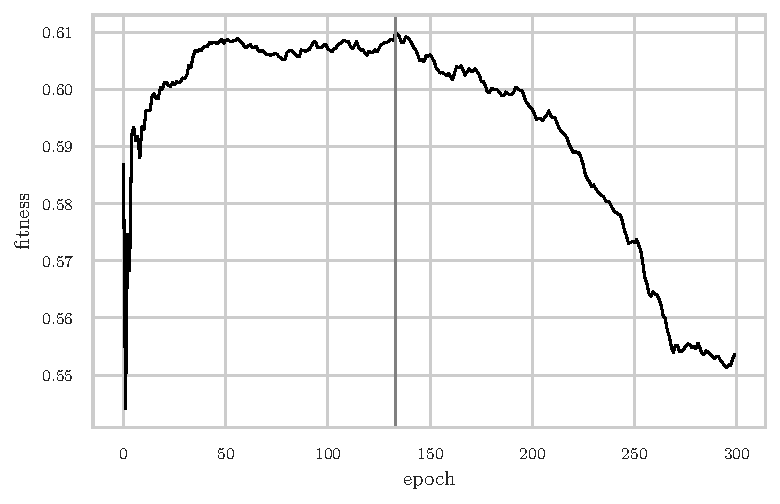
\includegraphics{graphics/model_fitness.pdf}
  \caption[Model fitness per epoch.]{Model fitness for each epoch
    calculated as in equation~\ref{eq:fitness}. The vertical gray line
    at 133 marks the epoch with the highest fitness.}
  \label{fig:fitness}
\end{figure}

Overall precision and recall per epoch are shown in
figure~\ref{fig:prec-rec}. The values indicate that neither precision
nor recall change materially during training. In fact, precision
starts to decrease from the beginning, while recall experiences a
barely noticeable increase. Taken together with the box and object
loss from figure~\ref{fig:box-obj-loss}, we speculate that the
pre-trained model already generalizes well to plant detection because
one of the categories in the COCO~\cite{lin2015} dataset is
\emph{potted plant}. Any further training solely impacts the
confidence of detection, but does not lead to higher detection
rates. This conclusion is supported by the increasing
\textsf{mAP}@0.5:0.95 until epoch 133.

\begin{figure}
  \centering
  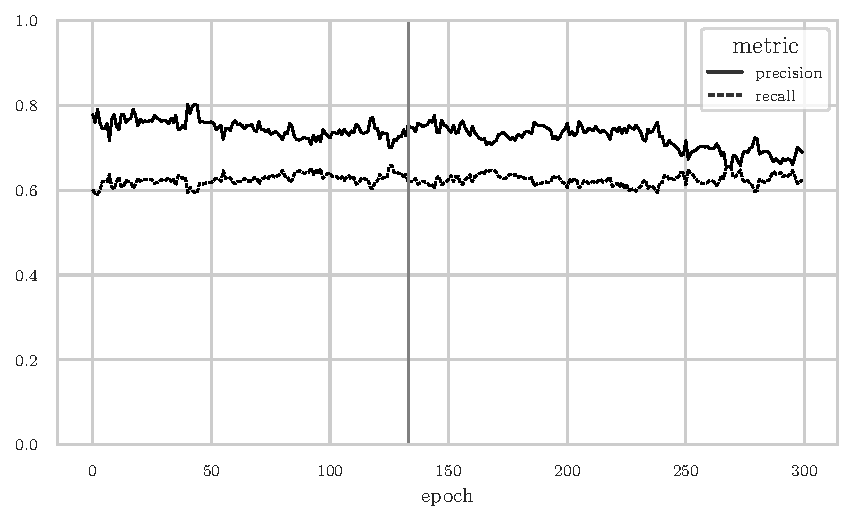
\includegraphics{graphics/precision_recall.pdf}
  \caption{Overall precision and recall during training for each
    epoch. The vertical gray line at 133 marks the epoch with the
    highest fitness.}
  \label{fig:prec-rec}
\end{figure}

Further culprits for the flat precision and recall values may be found
in bad ground truth data. The labels from the \gls{oid} are sometimes not
fine-grained enough. Images which contain multiple individual—often
overlapping—plants are labeled with one large bounding box instead of
multiple smaller ones. The model recognizes the individual plants and
returns tighter bounding boxes even if that is not what is specified
in the ground truth. Therefore, it is prudent to limit the training
phase to relatively few epochs in order to not penalize the more
accurate detections of the model. The smaller bounding boxes make more
sense considering the fact that the cutout is passed to the classifier
in a later stage. Smaller bounding boxes help the classifier to only
focus on one plant at a time and to not get distracted by multiple
plants in potentially different stages of wilting.

The box loss decreases slightly during training which indicates that
the bounding boxes become tighter around objects of interest. With
increasing training time, however, the object loss increases,
indicating that less and less plants are present in the predicted
bounding boxes. It is likely that overfitting is a cause for the
increasing object loss from epoch 40 onward. Since the best weights as
measured by fitness are found at epoch 133 and the object loss
accelerates from that point, epoch 133 is probably the correct cutoff
before overfitting occurs.

\begin{figure}
  \centering
  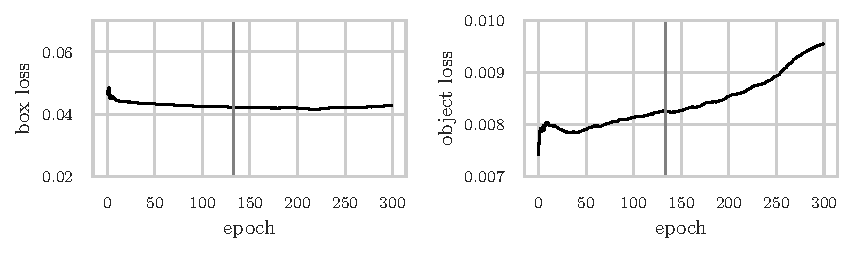
\includegraphics{graphics/val_box_obj_loss.pdf}
  \caption[Box and object loss.]{Box and object loss measured against
    the validation set of 3091 images and 4092 ground truth
    labels. The class loss is omitted because there is only one class
    in the dataset and the loss is therefore always zero.}
  \label{fig:box-obj-loss}
\end{figure}

\subsection{Test Phase}
\label{ssec:test-phase}

Of the 91479 images around 10\% were used for the test phase. These
images contain a total of 12238 ground truth
labels. Table~\ref{tab:yolo-metrics} shows precision, recall and the
harmonic mean of both (F1-score). The results indicate that the model
errs on the side of sensitivity because recall is higher than
precision. Although some detections are not labeled as plants in the
dataset, if there is a labeled plant in the ground truth data, the
chance is high that it will be detected. This behavior is in line with
how the model's detections are handled in practice. The detections are
drawn on the original image and the user is able to check the bounding
boxes visually. If there are wrong detections, the user can ignore
them and focus on the relevant ones instead. A higher recall will thus
serve the user's needs better than a high precision.

\begin{table}[h]
  \centering
  \begin{tabular}{lrrrr}
    \toprule
    {} &  Precision &    Recall &  F1-score &  Support \\
    \midrule
    Plant        &   0.547571 &  0.737866 &  0.628633 &  12238.0 \\
    \bottomrule
  \end{tabular}
  \caption{Precision, recall and F1-score for the object detection model.}
  \label{tab:yolo-metrics}
\end{table}

Figure~\ref{fig:yolo-ap} shows the \gls{ap} for the \gls{iou}
thresholds of 0.5 and 0.95. Predicted bounding boxes with an \gls{iou}
of less than 0.5 are not taken into account for the precision and
recall values of table~\ref{tab:yolo-metrics}. COCO's \cite{lin2015}
main evaluation metric is the \gls{ap} averaged across the \gls{iou}
thresholds from 0.5 to 0.95 in 0.05 steps. This value is then averaged
across all classes and called \gls{map}. The object detection model
achieves a state-of-the-art \gls{map} of 0.5727 for the \emph{Plant}
class.

\begin{figure}[h]
  \centering
  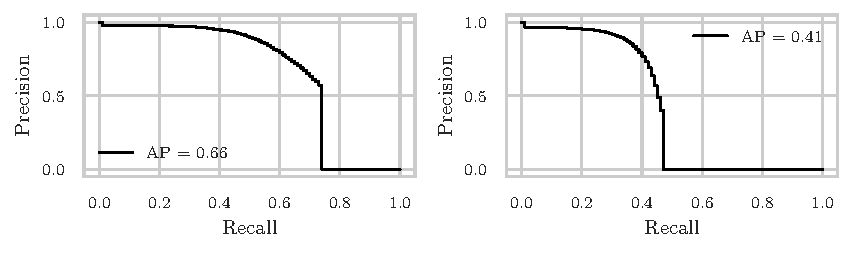
\includegraphics{graphics/APpt5-pt95.pdf}
  \caption[Object detection AP@0.5 and AP@0.95.]{Precision-recall
    curves for \gls{iou} thresholds of 0.5 and 0.95. The \gls{ap} of a
    specific threshold is defined as the area under the
    precision-recall curve of that threshold. The \gls{map} across
    \gls{iou} thresholds from 0.5 to 0.95 in 0.05 steps
    \textsf{mAP}@0.5:0.95 is 0.5727.}
  \label{fig:yolo-ap}
\end{figure}


\backmatter

% Use an optional list of figures.
\listoffigures % Starred version, i.e., \listoffigures*, removes the toc entry.

% Use an optional list of tables.
\cleardoublepage % Start list of tables on the next empty right hand page.
\listoftables % Starred version, i.e., \listoftables*, removes the toc entry.

% Use an optional list of alogrithms.
\listofalgorithms
\addcontentsline{toc}{chapter}{List of Algorithms}

% Add an index.
\printindex

% Add a glossary.
\printglossaries

% Add a bibliography.
\bibliographystyle{alpha}
\bibliography{references}

\end{document}
%%% Local Variables:
%%% mode: latex
%%% TeX-master: t
%%% End:
